This section solves Problem~\ref{prob:main} in two stages:
uncertainty-calibrated energy-based precedence cue (Sec.~\ref{sec:4.A}), and safety-preserving precedence integration (Sec.~\ref{sec:4.C}).
The overall procedure of our approach is summarized in Fig.~\ref{fig:method}.

\begin{figure*}[t!]
\centering
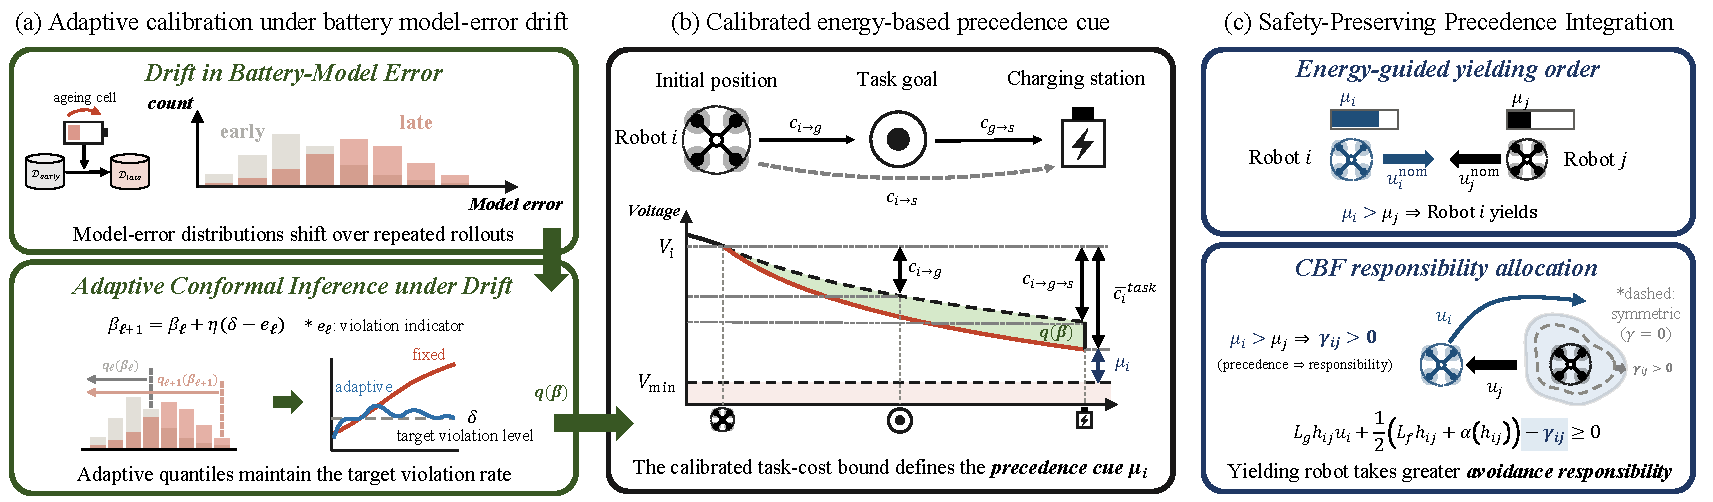
\includegraphics[width=\textwidth]{Figures/fig2.pdf}
\caption{Overview of the proposed energy-guided precedence framework. (a) Adaptive conformal inference calibrates battery-model error under distribution shift, producing an adaptive quantile $q_\ell(\beta_\ell)$ at the target violation level. (b) The calibrated task-cost bound defines the energy-based precedence cue $\mu_i$. (c) The resulting yielding order is encoded through CBF responsibility allocations, so the yielding robot assumes greater avoidance responsibility while pairwise safety is preserved.
\vspace{-10pt}
}
\label{fig:method}
\end{figure*}